\documentclass{article}
\usepackage[a4paper, margin=5em]{geometry}
\usepackage{fancyhdr}
\usepackage{lastpage}
\usepackage{graphicx}
\usepackage{hyperref}
%\usepackage{ngerman}
\usepackage{babel}
\usepackage{enumitem}
\usepackage{csquotes}
\usepackage{caption}
\usepackage{fancyvrb}
\usepackage{minted}
\usepackage{ulem}

\newcommand{\gqq}[1]{\glqq{}#1\grqq{}}

\pagestyle{fancy}
\fancyhf{}
\renewcommand{\headrulewidth}{0pt}
\setlength\parindent{0pt}
\fancyfoot{}

\lfoot{}
\cfoot{Seite \thepage\ / \pageref*{LastPage}}
\rfoot{}

\hypersetup{
    colorlinks=true,
    linktoc=all,
    urlcolor=blue
}

\author{Tim Wende}
\date{\today}
\title{\textbf{Hausaufgabe 9}}

\begin{document}
    \maketitle

    \newpage
    \section*{Builder Pattern}
    In der Vorlesung wurde das Builder Pattern \textbf{nicht} vorgestellt.

    \begin{enumerate}[label=\alph*.]
        \item Erklären Sie mit eigenen Worten, welchen Nutzen das Builder Pattern bringt und wo die typischen Einsatzgebiete liegen.
        
            Nutzen:
            Mit einem Builder kann man ein Objekt kontrolliert erstellen und nach jeder Operation die Qualität des theoretische Endresultats reevaluieren.
            So hat man jederzeit Kontrolle darüber, ob der jeweilige Anfragende das Objekt übergeben bekommt, oder ob der Builder als einziges eine Referenz erhalten darf.
            So muss ein Nutzender mit der API des Builders arbeiten, bis alle nicht optionalen Operationen durchgeführt wurden.
        
            typisches Einsatzgebiet:
            Builder sind nah verwandt mit Factories, wobei diese ein bisschen primitiver arbeiten.
            Sollte man im ctor verschiedene optionale Parameter\footnote{und man in der Sprache seiner Wahl keine default Werte hat. z.B. in Java} haben, entsteht hier ein sogenanntes \textbf{Telescoping Constuctor Pattern}.
            Dies sieht beispielsweise wie folgt aus (Spoilerwarnung: Aufgabenteil b.):

            \begin{minted}{java}
public Pokemon(String description){ ... }
public Pokemon(String description, Type type){ ... }
public Pokemon(String description, Type type, int hp){ ... }
public Pokemon(String description, Type type, int hp, int atk){ ... }

Pokemon p = new Pokemon("Glumanda", new Type("Feuer"), 39, 52);
            \end{minted}

            Hier sieht man, dass dies leicht unübersichtlich wird und man sich die Reihenfolge\footnote{und man in der Sprache seiner Wahl keine benannten Parameter hat. z.B. in Java} schwer merken kann.
            ist 39 \texttt{hp}? \texttt{atk}?
            Brauchen wir das?
            Was ist, wenn man nur \texttt{atk} und keine \texttt{hp} angeben möchte?
            Was ist, wenn \texttt{hp} von \texttt{atk} abhängig ist?
            Also zusammengefasst: das \textbf{Telescoping Constuctor Pattern} ist zu vermeiden!
            Aber wie?

            Die eben erwähnte Factory kann hier helfen, ist aber ebenfalls nicht wirklich schön:

            \begin{minted}{java}
PokemonFactory pf = new PokemonFactory();
Pokemon p =  pf.newPokemon("Glumanda");
p = pf.addType(p, new Type("Feuer"))
p = pf.addHP(p, 39)
p = pf.addATK(p, 52)
            \end{minted}

            Man sieht, dass \texttt{pf} über die gesamte Laufzeit immer wieder neu referenziert werden muss.
            Ebenso lässt sich der gesamte Vorgang nicht wirklich gut pipen, da wir ja auf dem Objekt selber arbeiten, und dieses die dort zu sehenden Methoden nicht kennt.

            Aber wie machen wir das jetzt gut?\footnote{Indem wir eine sinnvolle und gut Programmiersprache benutzen. z.B. nicht Java}
            In Java? Gar nicht.
            
            Aber der Builder kommt einem guten Endresultat doch schon ganz nah:

            \begin{minted}{java}
Pokemon p = new PokemonBuilder("Glumanda").with(new Type("Feuer")).withHP(39).withATK(52).build();
            \end{minted}

            Da jede Operation in diesem Prozess den Builder an sich zurückgibt, kann man hier das Pokemon \gqq{durchreichen}.
            Da man jedoch nie das Pokemon an sich in der pipe hat, sondern nur den Builder, ist es nicht möglich ein halb fertiges Objekt zu erhalten.
            Bei großen Sinnvollen implementierungen findet man in \texttt{.build()} vermehrt \texttt{.clone()} sowie eine Überprüfung auf Integrität und Qualität des Objekts an sich.
            Zusätzlich hat jedes \texttt{Pokemon} einen eigenenen, für sich selbst einzigartigen und zuständigen \texttt{PokemonBuilder}.

            Also zusammengefasst:
            \begin{itemize}
                \renewcommand\labelitemi{$\rightarrow$}
                \item Objekt mit optionalen Parametern: Telescoping Constuctor Pattern
                \item Zu viele Attribute: Factory
                \item Zu kompliziert: Builder
            \end{itemize}

            Also wenn man Objekte mit beliebig vielen, gleichartigen und optionalen Parametern im Konstruktor hat, welche kompliziert zu erstellen sind oder man die Integrität unter allen Umständen beibehalten möchte und die absolute Korrektheit des Objekts unentbehrlich wichtig ist, ist das Nutzen des Builder Patterns sinnvoll\footnote{wenn man in einer veralteten schlechten Programmiersprache schreibt. z.B. Java}.

        \newpage
        \item Finden Sie ein geeignetes Beispiel und erklären Sie dieses.
            Modellieren (Klassendiagramm) und \textbf{implementieren} Sie für diesen Anwendungsfall das Builder Pattern.

            Vorab: Eine gekürzte Version zur Überschaulichen Darstellung:
            \begin{figure}[ht]
                \centering
                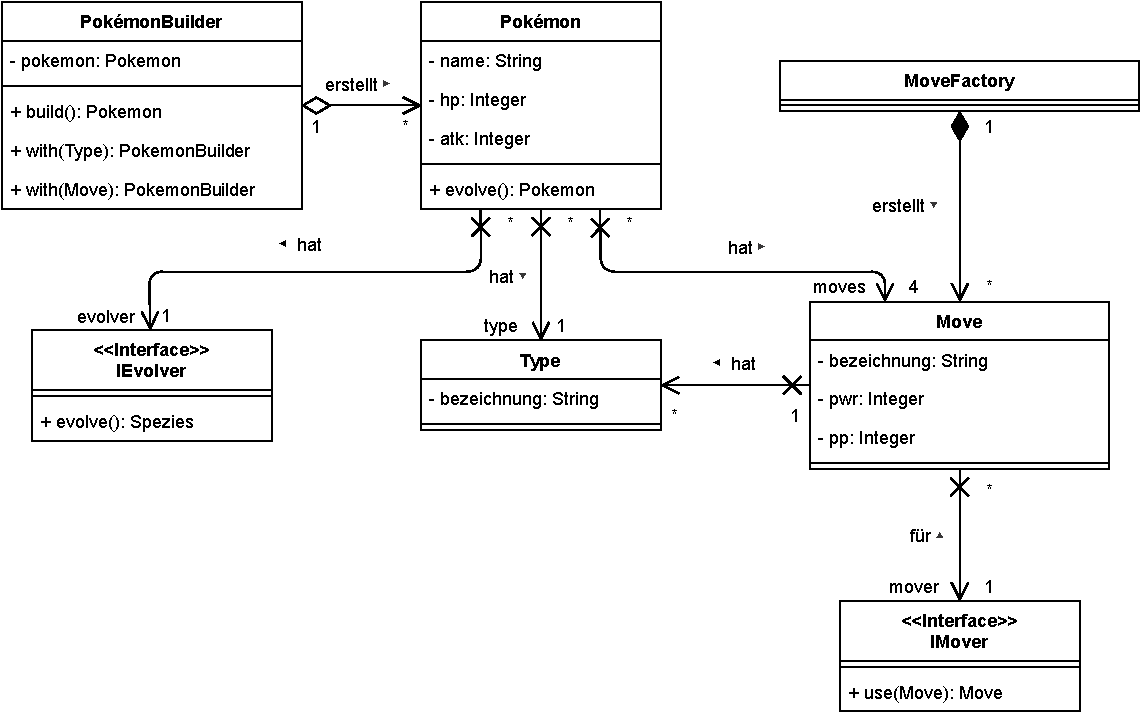
\includegraphics[width=0.75\textwidth]{swt_wende_tim_h09_class_diagram_simple.pdf}
                \caption{\texttt{class\_diagram\_simple}}
            \end{figure}

            Dieses Diagramm enthält einige Software Pattern:
            \begin{figure}[ht]
                \centering
                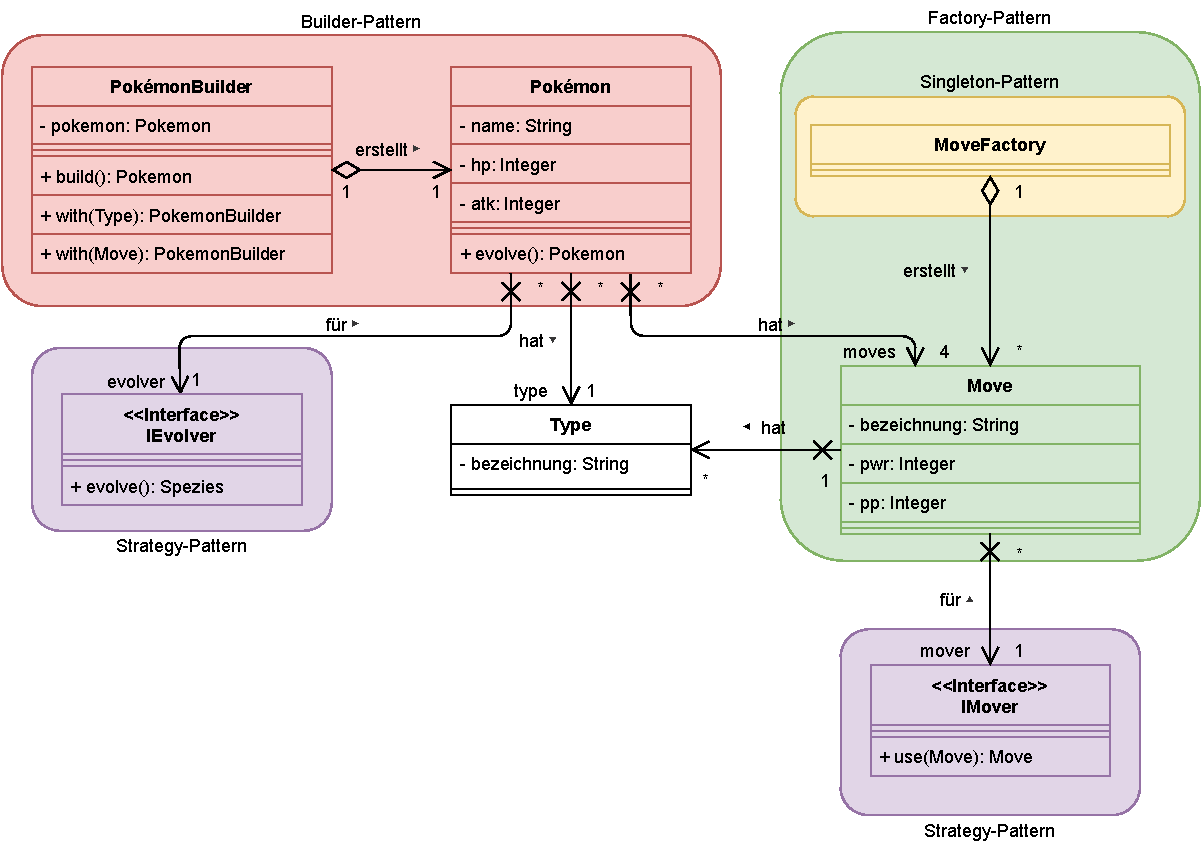
\includegraphics[width=0.75\textwidth]{swt_wende_tim_h09_class_diagram_pattern.pdf}
                \caption{\texttt{class\_diagram\_pattern}}
            \end{figure}

            Diese werden hoffentlich durch den Code verständlich dargestellt.

            \newpage
            Nun das Diagramm in voller Schönheit:
            \begin{figure}[ht]
                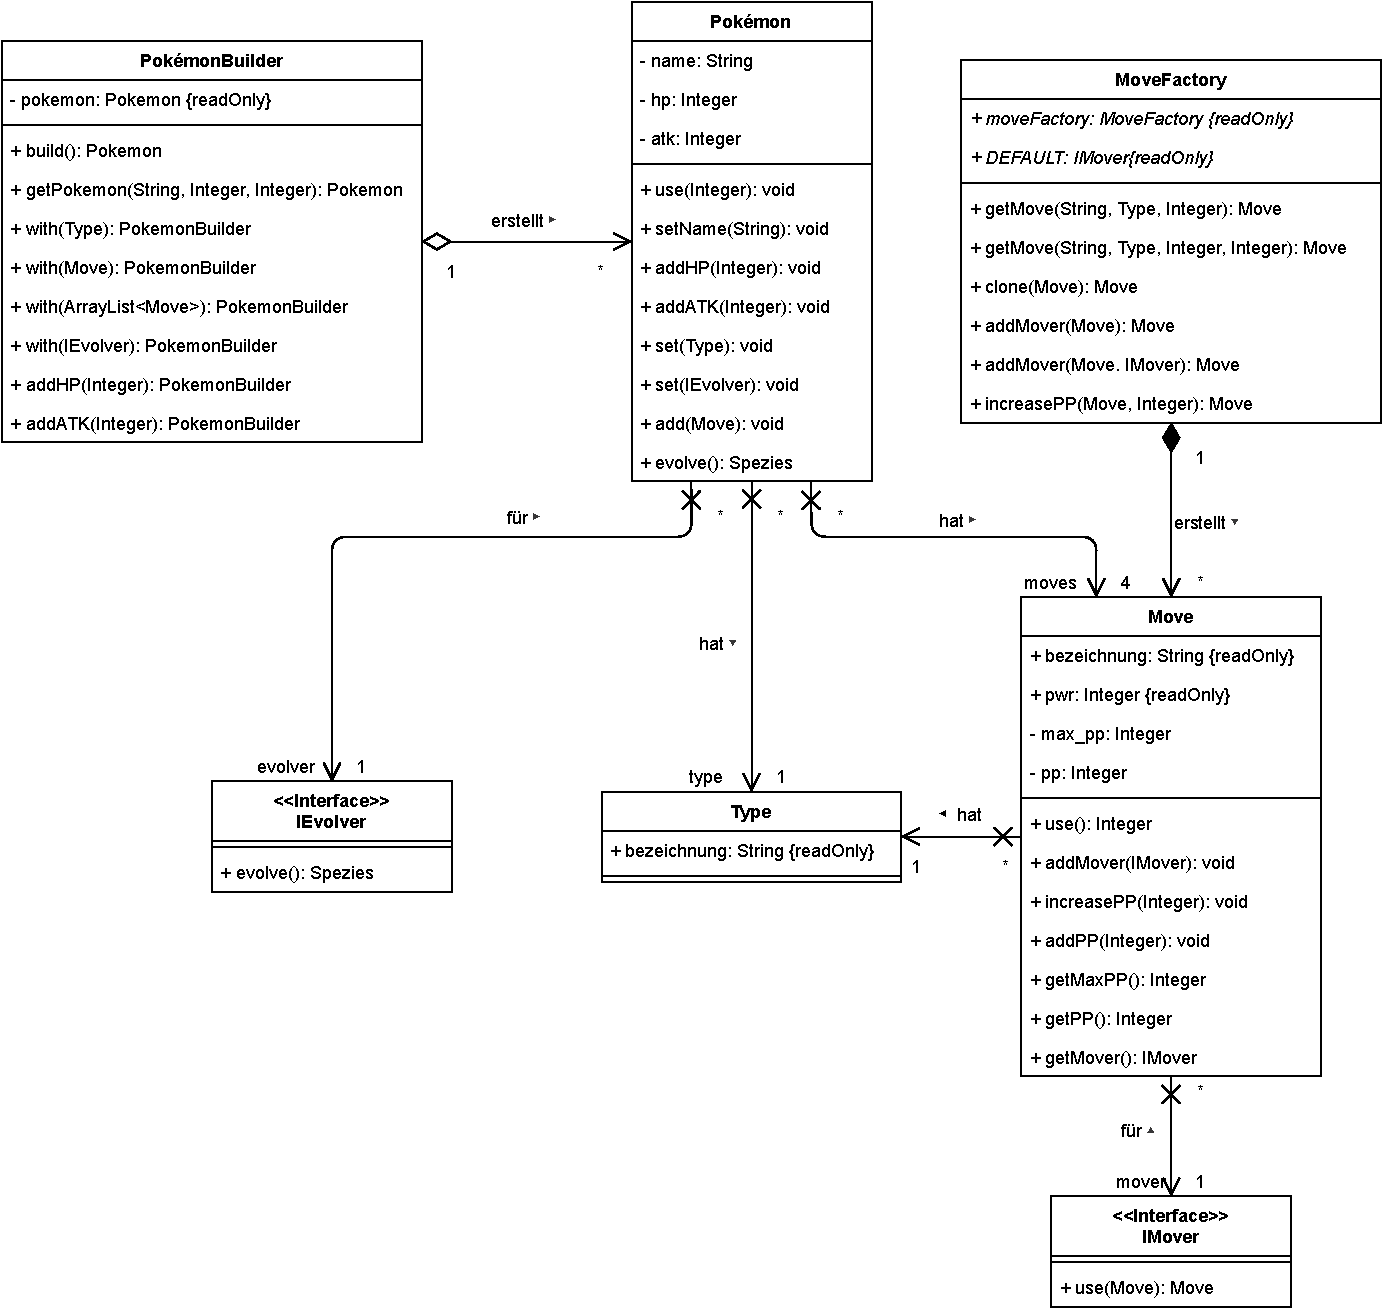
\includegraphics[width=\textwidth]{swt_wende_tim_h09_class_diagram.pdf}
                \caption{\texttt{class\_diagram}}
            \end{figure}

            \newpage
            Schauen wir uns nun die Main an:

            \inputminted{java}{Test.java}

            \newpage Diesen Code gehen wir nun einmal durch:

            \begin{minted}{java}
MoveFactory moveFactory = MoveFactory.moveFactory;
            \end{minted}

            Da wir nach dem Singleton Pattern handeln, wird hier eine Referenz auf das public Attribut in MoveFactory erstellt.
            Da dieses final ist, darf man gerne darauf zugreifen.\\

            \begin{minted}{java}
Type fire = new Type("Feuer");
            \end{minted}

            Type ist eine normale Klasse, hier ist nichts besonderes bei.\\

            \begin{minted}{java}
Move glut = moveFactory.addMover(
    moveFactory.increasePP(
        moveFactory.getMove(
            "Glut",
            fire,
            40
        ),
        25
    )
);
            \end{minted}

            Ich habe es mal versucht das Factory-Pattern schön darzustellen.
            Man nutzt, wie oben beschrieben, für jede Operation seine Factory:

            \begin{itemize}
                \item Zuerst erstellt man einen leeren Move:
                    \begin{minted}{java}
moveFactory.getMove("Glut", fire, 40);
                    \end{minted}

                \item Diesen übergibt man einen Betrag an AP:
                    \begin{minted}{java}
moveFactory.increasePP([...], 25);
                    \end{minted}

                \item Und lässt schlussendlich automatisch einen IMover hinzufügen:
                \begin{minted}{java}
moveFactory.addMover([...]);
                \end{minted}
            \end{itemize}

            Im letzten Schritt kann man ebenfalls einen eigenen IMover erstllen:

            \begin{itemize}
                \item z.B. wird hier wird (auf Grund eines Statuseffekts) jeder Schaden verdoppelt
                \begin{minted}{java}
moveFactory.addMover([...], move -> MoveFactory.DEFAULT.use(move) * 2);
                \end{minted}
            \end{itemize}

            Nun erstellen wir ein Pokemon:
            \begin{minted}{java}
Pokemon glumanda = new PokemonBuilder("Glumanda", 39, 52)
    .with(fire)
    .with(kratzer)
    .with(glut)
    .with(pokemon -> {
        String name = "Glutexo";
        System.out.println(pokemon + " entwickelt sich zu " + name);
        return new PokemonBuilder(name, pokemon).addHP(10).addATK(25).build();
    })
    .build();
            \end{minted}

            Bis zu \texttt{.build()} bearbeiten wir einen PokemonBuilder.
            Im Konstruktor geben wir alle nicht optionalen Parameter mit.
            Dann fügen wir ein Paar Attacken hinzu.
            Und zu guter Letzt erstellen wir ein Schema zum entwickeln.
            Dieses gibt einen Text aus und erstellt dank copy ctor ein neues Pokemon mit leicht erhöten Werten (ebenfalls mithilfe des PokemonBuilders).
    
            \newpage
            Unter Bezugnahme Ihres Kommentars zu Hausaufgabe 7 fallen alle weiteren Klassen ab hier weg.

            Jedoch hier einige Kommentare
            \begin{itemize}
                \item Das Builder-Pattern wurde in der Aggregation zwischen PokemonBuilder und Pokemon der Aufgabenstellung entsprechend realisiert
                \item Alle final Attribute sind public.
                    Dies öffnet natürlich Tür und Tor für jegliche Fehler, jedoch wollte ich dies nicht über-Engineeren
                \item Generell sind die Klassen offensichtlich Pokémon\texttrademark\hspace{0.1ex} nachempfunden, jedoch stark vereinfacht.
                    Auf fachliche Korrektheit sei bitte nicht zu achten.
                \item PokemonBuilder bearbeitet bis zu build ein private Pokemon.
                    Natürlich könnte man die Attribute von Pokemon ebenfalls im Builder nutzen, und so erst beim build() ein Pokemon erstellen.
                    Dies wäre sinnvoll, wenn der ctor aus Pokemon beispielsweise dieses einer public Liste hinzufügen sollte.
                    Da dies nicht der Fall ist, habe ich dies vernachlässigt.
                    Alternativ könnte man die Attribute über eine abstract Klasse verteilen, von der Beide Klasse erben.
                    Da \texttt{Java} jedoch nur von einer Klasse erben lässt, wollte ich diesen Platz nicht für einen solchen Unfug verschwenden.
                    Zusätzlich brauchte ich keine Überprüfung der qualitativen Korrektheit in build(), da alle verpflichtenden Attribute bereits im ctor des Builders gesetzt wurden.
                \item MoveFactory wirft im ctor einen Fehler, sollte dieser von außerhalb aufgerufen werden.
                    Explizit dieser sowie eventuell nicht nutzbare Konstruktoren sowie nicht zu erreichende Klassen sind public.
                    Von einer Lösung, welche eventuell durch Sichtbereiche abgesichterte Objekte, welche durch packages realisiert werden könnte oder sonstige Abhilfe bei diesem Problem habe ich abgesehen.
                    Durch hohe Kohäsion sind meine Klassen sowieso in einem einzigen package, da wäre dies auch schwierig umzusetzen.
                    Hilfreiche Methoden wie \texttt{friend} aus C++ zu imitieren war mir hier zu mühselig, jedoch durch \texttt{signature security} möglich.
            \end{itemize}

            Der Vollständigkeit halber, hier mein Output, welcher von der Test.main() erstellt wurde:
            \VerbatimInput{out.txt}
    \end{enumerate}

    \newpage
    \section*{Sequenzdiagramm: Wetterstation}
    In der Vorlesung haben Sie das Observer Pattern (zu deutsch Beobachter Entwurfsmuster) am Beispiel einer Wetterstation kennengelernt.
    Als Beispiel für konkrete Implementierungen der Interfaces Subject und Observer werden die Klassen \textit{WeatherData} bzw. \textit{CurrentConditionsDisplay} aus dem Foliensatz verwendet.\\

    Modellieren Sie in \sout{Visual Paradigm} \href{draw.io}{draw.io} ein Sequenzdiagramm, das diesen Sachverhalt darstellt.
    Das Diagramm soll die Interaktion der Klassen für den folgenden Programmablauf modellieren:

    \begin{enumerate}
        \item Eine Wetterstation startet und erstellt jeweils eine neue Instanz der Klassen \textit{WeatherData} und \textit{CurrentConditionsDisplay}.
            (Das Display bekommt die Wetterdaten im Konstruktor übergeben und registriert sich anschließend als Observer, siehe Folien)
        \item Es treten zwei Veränderungen des Wetters auf.
            Modellieren Sie einen Pull oder einen Push-Observer (Orientieren Sie sich an den Folien für einen Push-Observer)
        \item Der Observer wird vom Subject entfernt.
        \item Die Wetterstation wird abgeschaltet und der Speicher wird freigegeben
    \end{enumerate}

    \textbf{Hinweise:}
    \begin{itemize}
        \item Achten Sie zudem darauf, dass Methodenaufrufe innerhalb der selben Klasse richtig dargestellt werden.
        \item Benutzen Sie explizite Namen mit Typ für die Benennung der Teilnehmer.
        \item Benutzen Sie für Nachrichten die Form $<$Nachrichtenname$>$ ($<$Parametername$>$=$<$Argumentwert$>$,\dots)
    \end{itemize}

    
    \begin{figure}[ht]
        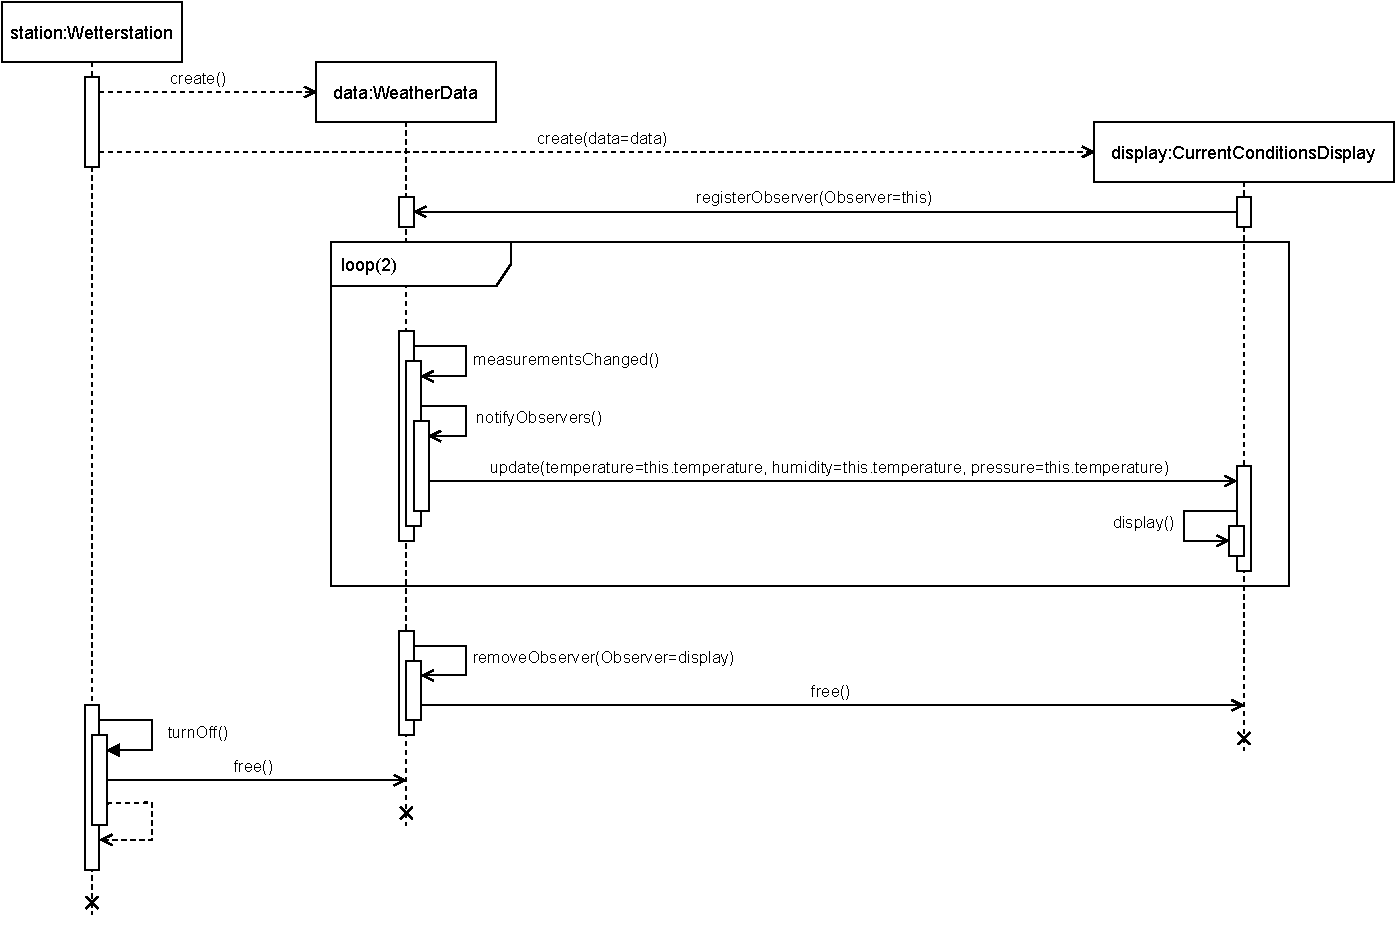
\includegraphics[width=\textwidth]{swt_wende_tim_h09_sequence_diagram.pdf}
        \caption{\texttt{sequence\_diagram}}
    \end{figure}
\end{document}